\documentclass[11pt]{article}
\usepackage[T1]{fontenc}
\usepackage[margin=1in]{geometry}
\usepackage{lmodern,microtype,amsmath,amssymb,booktabs,array}
\usepackage{tikz}
\usetikzlibrary{arrows.meta,positioning}
\usepackage[colorlinks=true,linkcolor=blue,urlcolor=blue,citecolor=blue]{hyperref}
\title{A Small-Scale, Auditable Recipe for Adapting a\newline 1.5B Language Model to Quantum-Chemistry Tasks}
\author{Project working draft}
\date{October 23, 2026}
\begin{document}
\maketitle
\begin{abstract}
Small local language models may help draft computational methods and inspect
scientific code, but fluent output can conceal elementary errors. We describe
a reproducible pilot and follow-up for adapting a 1.5-billion-parameter instruction model to
standard electronic-structure tasks on an 8\,GB Apple Silicon computer. The
first matched MLX experiment used 88 original training and 12 validation
examples with quantized-base low-rank adaptation. It completed 176 updates
in 130.34 seconds: reported validation loss decreased from 3.870 to 2.427,
but strict passes remained zero out of eight visible diagnostics before
and after adaptation. An expanded run added literature-informed exercises
and executed code examples, giving 144 training and 20 validation records.
Starting afresh from the same base, it completed 576 updates in 449.09
seconds. Validation loss decreased from 3.388 to 2.466, while strict passes
remained zero out of six different gradient and density-fitting diagnostics.
Truncations decreased within both experiments, without establishing reliable
scientific reasoning. The changed data, schedule and evaluation sets preclude
attributing a difference to dataset size alone. Reviews were unblinded and
performed by AI assistants, without independent human expert adjudication.
These runs demonstrate a feasible local training workflow and provide
auditable negative diagnostic results, not a reliable specialist model.
\end{abstract}

\section{Motivation and scope}
Electronic-structure methods combine mathematical conventions, physical
constraints, and implementation details. A useful writing assistant must
distinguish spin projection from total spin, state its density convention,
and use real program interfaces. A plausible-looking expression or a program
that parses is insufficient evidence of correctness. Standard references
provide the theoretical foundation \cite{helgaker}, while public PySCF
documentation and implementations connect theory to code \cite{pyscf,sun}.

We study a modest local adaptation task rather than a new electronic-structure
method. Qwen2.5-Coder-1.5B-Instruct supplies the starting instruction model
\cite{qwen}. Low-rank adaptation freezes most parameters and trains compact
updates \cite{lora}; quantized-base adaptation reduces the memory needed to
retain the frozen model \cite{qlora}. The experiments are designed for a
MacBook Air with an Apple M1 chip and 8\,GB unified memory. Hardware suitability
was verified by completed runs on this machine. This does not measure the
training memory high-water mark or establish performance on other hardware.

\section{Data construction and checks}
\subsection{Sources and task design}
The exercises cover spin, Hartree--Fock, configuration interaction,
multiconfigurational self-consistent field theory, orbital rotations,
finite-difference checks, and public PySCF interfaces. The data consist of
original Chinese and English questions and answers. Source books and papers
are not reproduced as a raw training corpus. Each exercise records source
identifiers and an explicit review status. Public code references identify
the local source version used for inspection, PySCF 2.6.2.

The first pilot contains 88 training and 12 validation records. Some records are
parameterized exercises, for example determinant-space dimensions or
nonredundant orbital-rotation counts. They increase coverage of constrained
problems without establishing independent scientific diversity. Twelve
validation records are excluded from training, but themes and references
overlap across splits.

\subsection{Verification}
We check JSONL structure, chat roles, nonempty answers, source resolution,
exact duplicate prompts, and length under the pinned chat tokenizer.
The first pilot's maximum observed training and validation lengths are 290 and 180 tokens,
respectively, below the 1024-token limit. Selected numerical checks
cover matrix exponentials, preservation of an AO metric, density traces,
and a finite-difference derivative. These checks do not certify all prose
or constitute independent expert review.

Eight diagnostic questions are stored separately from the training records.
Their prompts are distinct, but they were inspected during development and
the training data cover related concepts. We therefore treat them as a
transparent diagnostic set, not a blind benchmark or evidence of
source-disjoint generalization.

\section{Adaptation method}
Let $Q(W_0)$ denote a frozen, quantized linear map. For an adapted projection,
we write
\begin{equation}
 y = Q(W_0)x + sBAx,
 \qquad A\in\mathbb{R}^{r\times d_{\rm in}},\quad
 B\in\mathbb{R}^{d_{\rm out}\times r}.
\end{equation}
Only $A$ and $B$ are optimized. This equation uses column-vector notation;
the MLX implementation stores its factors in the corresponding transposed
layout. In MLX-LM, the configured scale $s$ multiplies the update directly.
It should not be interpreted as an alpha parameter that the framework will
automatically divide by $r$.

The base checkpoint is the MLX community four-bit conversion of
Qwen2.5-Coder-1.5B-Instruct, pinned to revision
\texttt{b3252a2f97102b1fb1571fec2c9b27219a8536be}.
Its configuration specifies group size 64. We use quantized-base LoRA in MLX,
not the original QLoRA paper's exact NF4 and paged-optimizer implementation.
Only query and value projections in the final four transformer blocks are
adapted. The final adapter tensor shapes contain 155,648 parameters,
consistent with the runtime report of approximately 0.156 million trainable
parameters. The adapter file occupies 624,302 bytes.

For example $i$ with answer-token positions $\mathcal A_i$, the intended
objective is a masked autoregressive cross-entropy,
\begin{equation}
 \mathcal L=-\frac{1}{\sum_i |\mathcal A_i|}
 \sum_i\sum_{t\in\mathcal A_i}
 \log p_{A,B}(y_{i,t}\mid x_i,y_{i,<t}).
\end{equation}
The training entry point supplies an explicit loss to both training and
validation. If the answer begins at token index $o$ in a sequence of length
$L$, supervised target indices satisfy $o\leq t<L$, excluding prompt and
padding tokens. The mask boundary is checked with a numerical example.
The fixed settings appear in
Table~\ref{tab:settings} for the first pilot. In each experiment, we select the final step in advance, without
selecting checkpoints by diagnostic answers.

\begin{table}[ht]
\centering
\caption{Fixed first-pilot configuration. These are settings, not measured outcomes.}
\label{tab:settings}
\begin{tabular}{ll}
\toprule
Parameter & Setting \\
\midrule
Training / validation examples & 88 / 12 \\
LoRA rank / direct MLX scale & 8 / 16 \\
Adapted modules & Query and value, final 4 blocks \\
Optimizer / learning rate & Adam / $10^{-4}$ \\
Batch size / optimizer steps & 1 / 176 \\
Sequence length limit & 1024 tokens \\
Validation interval & 44 steps, full validation set \\
Gradient checkpointing & Enabled \\
Random seed & 42 \\
\bottomrule
\end{tabular}
\end{table}

\begin{figure}[ht]
\centering
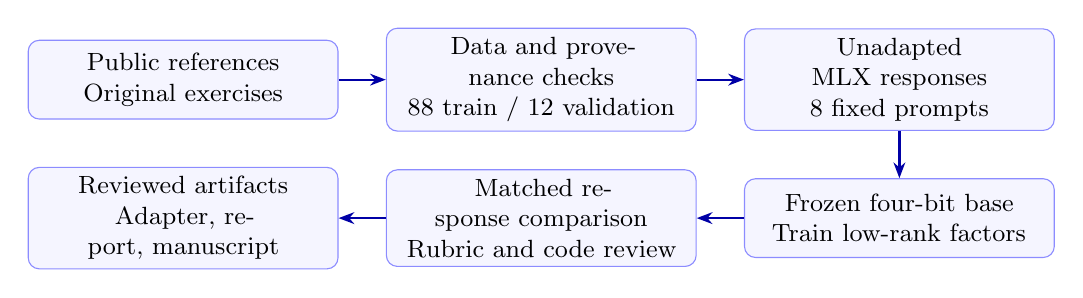
\begin{tikzpicture}[node distance=6mm and 6mm,
 box/.style={draw=blue!45,fill=blue!4,rounded corners,align=center,
 text width=3.7cm,minimum height=1.0cm,font=\small},
 arr/.style={-{Stealth[length=2mm]},thick,blue!65!black}]
\node[box] (source) {Public references\\Original exercises};
\node[box,right=of source] (data) {Data and provenance checks\\88 train / 12 validation};
\node[box,right=of data] (base) {Unadapted MLX responses\\8 fixed prompts};
\node[box,below=of base] (train) {Frozen four-bit base\\Train low-rank factors};
\node[box,left=of train] (eval) {Matched response comparison\\Rubric and code review};
\node[box,left=of eval] (release) {Reviewed artifacts\\Adapter, report, manuscript};
\draw[arr] (source)--(data);\draw[arr] (data)--(base);
\draw[arr] (base)--(train);\draw[arr] (train)--(eval);\draw[arr] (eval)--(release);
\end{tikzpicture}
\caption{First-pilot experimental workflow. The frozen branch retains public base
weights; the trainable branch learns answer-token supervision. The figure
describes the protocol; publication and deployment are separate from the
completed training experiment.}
\end{figure}

\section{Evaluation protocol and current observations}
\subsection{Exploratory baseline}
Before the matched MLX experiment, an exploratory Ollama run evaluated the
installed Qwen2.5-Coder:1.5b model in Q4\_K\_M format. It used temperature zero,
seed 42, a 2048-token context setting, and a maximum of 768 output tokens.
Table~\ref{tab:diagnostics} summarizes assistant-reviewed outcomes. Four
answers reached the output limit. Visible scientific errors are reported
separately from that truncation; a truncated response alone is not proof of
a particular conceptual error.

\begin{table}[ht]
\centering
\caption{Exploratory Ollama observations; not a before/after adaptation comparison.}
\label{tab:diagnostics}
\begin{tabular}{p{0.31\linewidth}p{0.57\linewidth}}
\toprule
Task & Observed outcome \\
\midrule
Electron counting & Violated the orbital-capacity constraint; truncated. \\
Matrix exponential & Repeated unsupported reasoning; truncated. \\
Weighted derivative & Omitted weight derivatives; truncated. \\
AO density metric & Incorrect metric contraction and idempotency criterion. \\
Operation-count analysis & Correctly withheld a speedup claim; incomplete rationale. \\
PySCF input & Invented key API names and did not perform the requested checks. \\
Missing mathematical context & Invented an expression; truncated. \\
Scientific claim restraint & Repeated unsupported priority and performance claims. \\
\bottomrule
\end{tabular}
\end{table}

None of the eight responses met all rubric items; one was partially correct.
This small, deliberately diagnostic sample cannot estimate overall model
quality. It also cannot be compared numerically with a later MLX run without
acknowledging differences in quantization, backend, and output budget.

\subsection{Matched first pilot}
The pipeline loads the same pinned MLX base model before and after
adaptation. Both stages use identical prompts and tokenizer settings,
greedy decoding, seed 42, and a 512-token output limit. It records complete
responses, stop reasons, token counts, elapsed time and peak memory.
The final adapter is fixed by iteration count, not by the diagnostic score.
Evaluation must distinguish correctness, partial completion, hallucinated
interfaces, repetition and truncation. Generated code is not executed
automatically.

\begin{table}[ht]
\centering
\caption{Measured first-pilot outcomes. Strict passes require the complete
rubric and no materially contradictory scientific claim.}
\begin{tabular}{lll}
\toprule
Measurement & Before & After \\
\midrule
Strict diagnostic passes & 0/8 & 0/8 \\
Token-limit truncations & 6/8 & 2/8 \\
Total generated diagnostic tokens & 3,174 & 1,786 \\
Reported inference peak (GB) & 1.145 & 1.145 \\
\bottomrule
\end{tabular}
\end{table}

The native-terminal run completed on October 23, 2026. Stage wall times,
including each subprocess's setup, were 62.32 seconds for baseline inference,
130.34 seconds for training, and 34.69 seconds for adapted inference. Inference
times differ partly because answer lengths changed and are not a speedup
benchmark. Training peak memory was not recorded. The inference values are
MLX process high-water reports and do not measure total system memory.

Reported validation losses at iterations 1, 44, 88, 132, and 176 were 3.870,
3.186, 2.792, 2.509, and 2.427. These teacher-forced losses declined while
strict scientific correctness on the eight visible diagnostics did not
improve. The adapted model rejected a quartet for the electron-count task
but supplied an incorrect spin argument. Its weighted derivative was wrong;
its density code substituted $D^2$ for $DSD$. The program-generation answer
still placed both hydrogen nuclei at the same position and invented
convergence attributes. Unsupported method and priority claims persisted.
The matrix-exponential answer merely described a plan without solving the
problem. All raw responses and the unblinded AI-assisted review are included.

The shorter outputs and fewer truncations show a change in response behavior,
not demonstrated scientific reliability. No checkpoint was selected from
these diagnostic results. The follow-up below is a separate experiment;
its outcomes do not replace or revise this pilot's reported scores.

\subsection{Expanded follow-up}
We expanded the exercises using additional public literature and PySCF
interfaces \cite{pyscf2020}. The 64 added records comprise 56 training and
eight validation examples, bringing the totals to 144 and 20. They include
methods paragraphs, code repairs and interpretations of actual numerical
outputs. Twelve original numerical cases were executed with PySCF 2.6.2,
NumPy 2.5.4 and SciPy 1.18.1; all their assertions passed. Nine code families
enter training: RHF, UHF, MP2, CCSD, CASCI, CASSCF, AO-to-MO integral
transformation, generalized eigenproblems and DIIS. Rayleigh--Ritz examples
enter validation. Nuclear-gradient and density-fitting cases are excluded
from the newly added training examples and supply six diagnostic prompts.
The original pilot records remain included, and broad concepts can overlap.
The diagnostic questions and reference code were visible to the AI assistant
during development, so this family separation is not a blind benchmark.
Passing assertions in the authored examples does not validate generated code.

This run starts afresh from the same pinned base, without continuing the
pilot adapter. Seed 42, adapter rank and direct scale, block placement,
optimizer, learning rate, answer-only loss, batch size and sequence limit
remain unchanged. The fixed schedule is 576 updates, or four nominal passes
through the training records, with full validation every 144 steps. Maximum
training and validation lengths are 479 and 402 tokens. Before and after
inference use the same six prompts and the same decoding protocol as above.
The fixed final adapter is evaluated, without diagnostic-based checkpoint
selection.

\begin{table}[ht]
\centering
\caption{Matched follow-up outcomes on six development-visible diagnostics.
These cases differ from the first pilot's eight questions.}
\label{tab:followup}
\begin{tabular}{lll}
\toprule
Measurement & Before & After \\
\midrule
Strict diagnostic passes & 0/6 & 0/6 \\
Token-limit truncations & 3/6 & 1/6 \\
Total generated diagnostic tokens & 2,766 & 1,312 \\
Reported inference peak (GB) & 1.173 & 1.172 \\
\bottomrule
\end{tabular}
\end{table}

The follow-up completed on October 23, 2026. Stage times were 53.31 seconds
for baseline inference, 449.09 seconds for training and 28.64 seconds for
adapted inference, including subprocess setup. Reported validation losses
at iterations 1, 144, 288, 432 and 576 were 3.388, 2.769, 2.578, 2.495 and
2.466. Training peak memory was again not measured; the approximately
1.173\,GB inference reports are not training or total-system memory.

Strict passes remained zero (Table~\ref{tab:followup}). The adapted model
omitted the numerical gradient and force in the first task and invented a
unit-conversion factor in the second. Its gradient-code response repeated
a dependency list until truncation. It miscomputed the density-fitting
energy difference, omitted a requested verification workflow, and restated
the final code-generation request without implementing it. The primary AI
assistant and a separate AI reviewer agreed on the strict pass outcomes;
this was unblinded AI review, not independent human expert adjudication.
Generated code was not executed automatically. Raw responses, review reasons
and measured metrics are retained separately from the first pilot.

Both the data and the training duration changed, so this experiment does
not isolate an effect of adding literature or code. The validation records
and diagnostic sets also changed: their losses and scores must not be used
as a direct between-experiment ranking. Within the follow-up, lower loss
and fewer truncations again did not establish reliable scientific answers.

\section{Limitations and reproducibility}
The dataset is small, partly templated, and authored and reviewed by an AI
assistant rather than an independent expert panel. Validation and diagnostic
items share topics with training, and the diagnostic questions influenced
development priorities. Each experiment uses one seed, with no seed replicates,
no model-size comparison,
and no broad forgetting or out-of-domain evaluation. Loss reduction would
not by itself establish reliable derivation or code generation.

The repository includes the fixed configuration, model revision, dependency
lock, data generator, per-example provenance, evaluation scripts, vector
workflow figure, input hashes, actual logs, responses and adapter files.
Machine-local paths in the distributed adapter configuration and log have
been replaced by portable paths without changing the trained weight bytes.
Further work should include expert adjudication,
unseen molecules and algorithm families, code-execution tests, multiple
seeds, and a source-disjoint evaluation set. Any eventual improvement must
be stated at the level supported by those tests.

\paragraph{Local deployment.}
The first-pilot adapter was also merged with the pinned base by CPU affine
dequantization and FP16 low-rank addition, converted using llama.cpp release
b11836, requantized to Q4\_K\_M, and imported into Ollama 0.40.6.
Loading and a generation call succeeded, but the separate smoke response
misstated basic spin concepts. This checks deployability only. CPU fusion
was not verified bitwise against native MLX fusion, and further quantization
can change outputs; the matched MLX scores above do not characterize this
deployment export. The follow-up export also loaded successfully, but its
smoke response misstated total spin and repeated to the token limit.
Both exports' hashes and raw responses are recorded in the repository.

\paragraph{Disclosure.}
The dataset, scripts and manuscript were prepared with AI assistance.
This document is an unsubmitted working draft. It reports no new
electronic-structure algorithm and makes no claim of expert-level reliability.

\begingroup
\footnotesize
\begin{thebibliography}{9}
\setlength{\itemsep}{2pt}
\setlength{\parskip}{0pt}
\bibitem{helgaker} T. Helgaker, P. J\o rgensen and J. Olsen.
\emph{Molecular Electronic-Structure Theory}. Wiley, 2000.
\bibitem{pyscf} PySCF developers. Multi-configuration self-consistent field documentation.
\url{https://pyscf.org/user/mcscf.html}. Accessed October 23, 2026.
\bibitem{sun} Q. Sun, J. Yang and G. K.-L. Chan.
A general second order complete active space self-consistent-field solver for large-scale systems.
\emph{Chemical Physics Letters} 683, 291--299 (2017).
\url{https://doi.org/10.1016/j.cplett.2017.03.004}.
\bibitem{pyscf2020} Q. Sun et al. Recent developments in the PySCF program package.
\emph{Journal of Chemical Physics} 153, 024109 (2020).
\url{https://doi.org/10.1063/5.0006074}.
\bibitem{qwen} B. Hui et al. Qwen2.5-Coder Technical Report.
arXiv:2409.12186 (2024). \url{https://arxiv.org/abs/2409.12186}.
\bibitem{lora} E. J. Hu et al. LoRA: Low-Rank Adaptation of Large Language Models.
arXiv:2106.09685 (2021). \url{https://arxiv.org/abs/2106.09685}.
\bibitem{qlora} T. Dettmers, A. Pagnoni, A. Holtzman and L. Zettlemoyer.
QLoRA: Efficient Finetuning of Quantized LLMs.
arXiv:2305.14314 (2023). \url{https://arxiv.org/abs/2305.14314}.
\bibitem{mlx} MLX-LM developers. Fine-Tuning with LoRA or QLoRA.
\url{https://github.com/ml-explore/mlx-lm/blob/main/mlx_lm/LORA.md}.
Implementation inspected: MLX-LM 0.32.2.
\end{thebibliography}
\endgroup
\end{document}
